This section serves as an introduction of tensor network manipulations. The overview mainly focusses on MPS/MPO networks, but most of the oprations translate to the 2D case.

The MPS's are processed by transforming the tensor into a matrix, performing some matrix calculations and casting it back into its original form. In this way, the standard methods from linear algebra can be used. This section gives some examples how this is done in practice:

\subsection{Basics}

\subsubsection{Grouping legs}
One of the most basic manipulations is to group some legs of a tensor into one leg:
\begin{equation}
    \begin{split}
        T^{i_1 i_2 j_1 j_2} &=  \expH{2}{$T$}{{"$i_1$","$i_2$"}}{{"$j_1$","$j_1$"}}{} \\
        & \cong \expH{2}{$T$}{{"-","-"}}{{"-","-"}}{{"$(i_1 j_1 )$","$(i_2 j_2)$"}} \\
        &= T^{ (i_1 j_1 ) (i_2 j_2) } \\
    \end{split}
\end{equation}
The dimension of the new leg is the product of the dimension of the individual legs. Contracting 2 merged legs with 2 merged legs is exactly the same as contracting them separately. The both The 4 leg tensor and matrix contain exactly the same information.
Manipulating this in memory requires both permute and reshape commands. This requires some time, the internal representation of the matrix changes.

\subsubsection{decomposition} \label{decompMPO}

The grouping above can be applied to decompose a tensor into 2 tensor with matrix techniques. An example, which will be needed later on, is give here.

\def \figone {\expH{2}{$O^{u v,v w}$}{{"$i_1$","$i_2$"}}{{"$j_1$","$j_1$"}}{{"u","w"}}}

\begin{equation}
    \begin{split}
        \figone &= O^{i_1 i_2 j_1 j_2 }_{\alpha_u \gamma_w} \\
        &\cong O^{u w}_{ (\alpha_u i_1 j_1) (\gamma_w i_2 j_2) } \\
        &= O^{u v}_{(\alpha_u i_1 j_1) \alpha_v } O^{v w}_{ \alpha_v (\alpha_w i_2 j_2) } \\
        &\cong \mpo{2}{{"u","v","w"}}{{"$i_1$","$i_2$"}}{{"$j_1$","$j_1$"}}{}{}
    \end{split}
\end{equation}

The indices U,V and W represent blocks indices. Step 2 reshapes and groups the indices on to one index on the left and one on the right. The dimension of this index is the product of the separate dimensions. Step 3 decomposes the matrix into a product of 2 matrices. The last step transforms the indices back to separate legs.

For an exact representation, the bond dimension of virtual level v is:
\begin{equation}
    \dim{v} = \min( \dim{u}, \dim{v}) + 2 \dim{i}
\end{equation}

Many matrix decompositions exist. Some useful examples here are SVD decomposition, eigenvalue decomposition, QR, $\cdots$.

\subsubsection{virtual levels}
In the previous example, the levels were indicate with a block index or virtual level. The idea is to create seperate the contraction into blocks. This is completely analogous to matrix block multipliction. This wil be a more natural form to represent the algorithm. Of course, one can easily switch between block representation and the full one.

\subsubsection{inverse}
Suppose we want to find a MPO O for given tensors A and B such that the following holds:

\def \figone {\expH{2}{$A$}{{"$i_1$","$i_2$"}}{{"$j_1$","$j_2$"}}{{"u",}}}
\def \figthree {\expH{3}{$B$}{{"$i_1$","$i_2$","$i_3$"}}{{"$j_1$","$j_2$","$j_3$"}}{{"u","v"}}}

\def \figtwo {\mpo{1}{{,"v"}}{{"$i_3$",}}{{"$j_3$",}}{}{}}

\begin{equation}
    \combineTikz{ \figone }{\figtwo}{1.8} =  \figthree
\end{equation}

Again, the indices can be taken toghether in the following way: $\alpha = (u i_1 j_1  i_2 j_2)$ and $\beta = (i_3 j_3 v)$:
\begin{equation}
    A_{\alpha \gamma} O_{\gamma \beta} = B_{\alpha \beta}
\end{equation}
This a a standard matrix equation and can hence be solved with linear algebra packages. Note that it is not necessary to calculate $A^{-1}$ to obtain the solution. Linear solver are generally much faster. As this is one of the core problems to solve both in 1D and 2D, this will be discussed in detail in \cref{sec:framework_impl}.

\subsubsection{contraction order}

\todo{contraction order}

\subsubsection{Gauge freedom}

\todo{gauge}
\subsubsection{truncation}

\todo{svd truncation}

\subsection{MPS algoritms}

%https://arxiv.org/pdf/1306.2164.pdf

\subsubsection{cononical form}

schmidt decomp,

\subsubsection{DMRG}

\subsubsection{Expectation values}

Suppose that the there is an MPO representation of $ e^{ - \beta \hat{H} } $ A and that the mpo represenation for X Y is localised over n sites, then the expactation value is given by:

\begin{equation}
    \Braket{X} = \frac{
        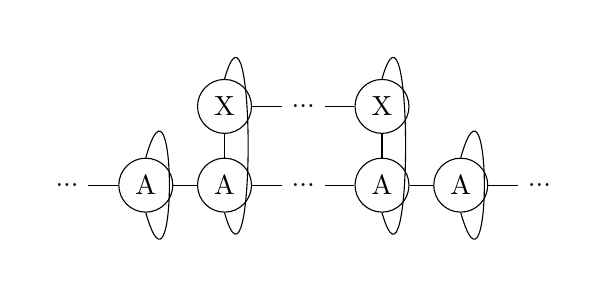
\begin{tikzpicture} [   ]
            \clip (-1.5,-1) rectangle (5.5,2);

            \node[] (N0) at (-1,0) {...};
            \node[circle, draw] (N1) at (0,0) {A};
            \node[circle, draw] (N2) at (1,0) {A};
            \node[circle, draw] (X2) at (1,1) {X};

            \node[] (N3) at (2 ,0) {...};
            \node[] (X3) at (2,1) {...};

            \node[circle, draw] (N4) at (3 ,0) {A};
            \node[circle, draw] (X4) at (3,1) {X};

            \node[circle, draw] (N5) at (4 ,0) {A};
            \node[] (N6) at (5 ,0) {...};

            \draw  (N0) -- (N1) ;

            \draw  (N1) -- (N2) ;
            \draw  (N2) -- (N3) ;
            \draw  (N3) -- (N4) ;
            \draw  (N4) -- (N5) ;
            \draw  (N5) -- (N6) ;

            \draw  (X2) -- (X3) ;
            \draw  (X3) -- (X4) ;

            \draw  (N2) -- (X2) ;
            \draw  (N4) -- (X4) ;

            \draw (X2.north)   .. controls +(0.4,1.4) and +(0.4,-1.4) .. (N2.south);
            \draw (X4.north)   .. controls +(0.4,1.4) and +(0.4,-1.4) .. (N4.south);

            \draw (N1.north)   .. controls +(0.4,1.4) and +(0.4,-1.4) .. (N1.south);
            \draw (N5.north)   ..  controls +(0.4,1.4) and +(0.4,-1.4)  .. (N5.south);
        \end{tikzpicture}
    }{
        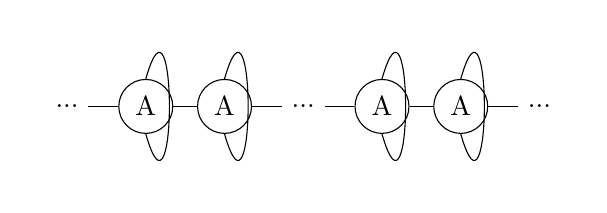
\begin{tikzpicture} [   ]

            \clip  (-1.5,-3) rectangle (5.5,-1);

            \node[] (O0) at (-1,-2) {...};
            \node[circle, draw] (O1) at (0,-2) {A};
            \node[circle, draw] (O2) at (1,-2) {A};

            \node[] (O3) at (2 ,-2) {...};
            \node[circle, draw] (O4) at (3 ,-2) {A};

            \node[circle, draw] (O5) at (4 ,-2) {A};
            \node[] (O6) at (5 ,-2) {...};

            \draw  (O0) -- (O1) ;

            \draw  (O1) -- (O2) ;
            \draw  (O2) -- (O3) ;
            \draw  (O3) -- (O4) ;
            \draw  (O4) -- (O5) ;
            \draw  (O5) -- (O6) ;

            \draw (O2.north)   .. controls +(0.4,1.4) and +(0.4,-1.4) .. (O2.south);
            \draw (O4.north)   .. controls +(0.4,1.4) and +(0.4,-1.4) .. (O4.south);

            \draw (O1.north)   .. controls +(0.4,1.4) and +(0.4,-1.4) .. (O1.south);
            \draw (O5.north)   ..  controls +(0.4,1.4) and +(0.4,-1.4)  .. (O5.south);
        \end{tikzpicture}
    }
    \label{sm:expecatation_X}
\end{equation}

In the thermodynamic limit there are an infinity number of A to the left and the right. This can be simulated by taking the left and right fixed points of the traced MPO A corresponding to the largest eigenvector $\lambda$.

\begin{equation}
    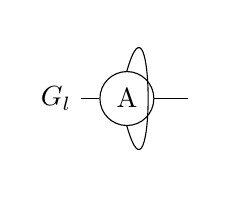
\begin{tikzpicture}[baseline={0cm-0.5*height("$=$")} , scale=0.9]
        \clip (-1.4,-1) rectangle (1,1);
        \node[] (N0) at (-1,0) {$G_l$};
        \node[] (N2) at (1,0) {};
        \node[circle, draw] (N1) at (0,0) {A};
        \draw  (N0) -- (N1) ;
        \draw  (N1) -- (N2) ;
        \draw (N1.north)   .. controls +(0.4,1.4) and +(0.4,-1.4) .. (N1.south);
    \end{tikzpicture}
    = \lambda
    \begin{tikzpicture}[baseline={0cm-0.5*height("$=$")}, scale=0.9 ]
        \clip (-.4,0.5) rectangle (1,-0.5);
        \node[] (N2) at (1,0) {};
        \node[] (N1) at (0,0) {$G_l$};
        \draw  (N1) -- (N2) ;
    \end{tikzpicture}
\end{equation}

\begin{equation}
    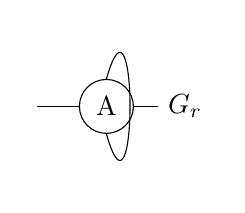
\begin{tikzpicture}[baseline={0cm-0.5*height("$=$")} ]
        \clip (-1,-1) rectangle (1.4,1);
        \node[] (N0) at (-1,0) {};
        \node[] (N2) at (1,0) {$G_r$};
        \node[circle, draw] (N1) at (0,0) {A};
        \draw  (N0) -- (N1) ;
        \draw  (N1) -- (N2) ;
        \draw (N1.north)   .. controls +(0.4,1.4) and +(0.4,-1.4) .. (N1.south);
    \end{tikzpicture}
    = \lambda
    \begin{tikzpicture}[baseline={0cm-0.5*height("$=$")} ]
        \clip (0,-0.5) rectangle (1.4,0.5);
        \node[] (N2) at (1,0) {$G_l$};
        \node[] (N1) at (0,0) {};
        \draw  (N1) -- (N2) ;
    \end{tikzpicture}
\end{equation}

Equation \cref{sm:expecatation_X} can now be easily caclulated:

\begin{equation}
    \Braket{X} = \frac{
        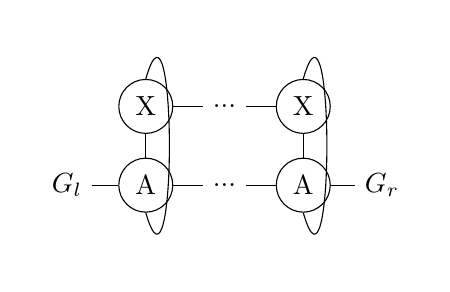
\begin{tikzpicture} [   ]
            \clip (-0.5,-1) rectangle (4.5,2);

            \node[] (N1) at (0,0) {$G_l$};
            \node[circle, draw] (N2) at (1,0) {A};
            \node[circle, draw] (X2) at (1,1) {X};

            \node[] (N3) at (2 ,0) {...};
            \node[] (X3) at (2,1) {...};

            \node[circle, draw] (N4) at (3 ,0) {A};
            \node[circle, draw] (X4) at (3,1) {X};

            \node[] (N5) at (4 ,0) {$G_r$};

            \draw  (N1) -- (N2) ;
            \draw  (N2) -- (N3) ;
            \draw  (N3) -- (N4) ;
            \draw  (N4) -- (N5) ;

            \draw  (X2) -- (X3) ;
            \draw  (X3) -- (X4) ;

            \draw  (N2) -- (X2) ;
            \draw  (N4) -- (X4) ;

            \draw (X2.north)   .. controls +(0.4,1.4) and +(0.4,-1.4) .. (N2.south);
            \draw (X4.north)   .. controls +(0.4,1.4) and +(0.4,-1.4) .. (N4.south);

        \end{tikzpicture}
    }{
        \lambda^n
        \begin{tikzpicture}[baseline={0cm-0.5*height("$=$")} ]
            \clip (-0.5,-0.5) rectangle (1.4,0.5);
            \node[] (N2) at (1,0) {$G_r$};
            \node[] (N1) at (0,0) {$G_r$};
            \draw  (N1) -- (N2) ;
        \end{tikzpicture}
    }
    \label{sm:expecatation_X_2}
\end{equation}

